\documentclass[12pt]{article}
\usepackage[margin=1in]{geometry}
\usepackage{amsmath,amssymb}
\usepackage{graphicx}
\usepackage{hyperref}
\usepackage{enumitem}
\usepackage{caption}
\usepackage{setspace}
\onehalfspacing
\graphicspath{{../../static/screenshots/}}

\title{专利二：黏菌-量子联合路径追踪与拓扑识别方法与系统}
\author{申请人：ChainAML 项目}
\date{\today}

\begin{document}
\maketitle

\begin{abstract}
提出一种结合黏菌仿生优化与量子搜索的路径追踪方法，使用“用进废退”强化主路径并在疑似节点施加陷阱吸引，再以量子幅度放大在候选路径集中放大高风险路径，适配复杂“分层-回流-再分散”的洗钱拓扑。
\end{abstract}

\section*{技术领域}
图优化、仿生算法与量子搜索交叉领域。

\section*{背景技术}
传统最短路或静态规则在大规模图上的隐匿资金路径识别能力不足。

\section*{发明内容（概要）}
黏菌导通性演化 + 陷阱吸引 + 量子搜索联合框架，提高高风险路径检出效率与拓扑定位能力。

\section*{附图说明}
图3：联合流程图。\\
图4：路径可视化（随机静脉与加粗主路径）。\\
图5：Step II 页面截图占位。

\section*{具体实施方式}
\subsection*{图模型与参数}
地址交易图 $G=(V,E)$；初始导通性 $C_{ij}(0)$；节点势 $P_i$。参数：$\alpha,\beta,\delta,\gamma,\eta$。

\subsection*{黏菌导通性演化}
流强度（压差流近似）：
\begin{equation}
Q_{ij}=\gamma (P_i-P_j)
\end{equation}
导通性更新：
\begin{equation}
C_{ij}(t+1)=(1-\alpha)C_{ij}(t)+\beta |Q_{ij}|-\delta\cdot \mathbf{1}_{\text{unused}}
\end{equation}

\subsection*{陷阱吸引}
对陷阱节点 $h\in H$ 施加势或强化参数：
\begin{equation}
\tilde{P}_h=P_h-\eta,\ \ \beta' > \beta \ \text{针对经过陷阱的边}
\end{equation}

\subsection*{量子搜索（候选路径集）}
初态：
\begin{equation}
|s\rangle=\frac{1}{\sqrt{N}}\sum\limits_{p\in \text{Paths}}|p\rangle
\end{equation}
Oracle 标记高风险路径集 $\mathcal{M}$ 并相位翻转；扩散算子：
\begin{equation}
D=2|s\rangle\langle s|-I
\end{equation}
迭代 $r$ 次后命中概率：
\begin{equation}
\Pr(\text{hit})=\sin^2((2r+1)\theta),\ \ \text{其中}\ \ \sin^2\theta=\frac{|\mathcal{M}|}{N}
\end{equation}

\subsection*{实施环境与数据}
同专利一说明；陷阱集合从混币器/提现节点与时间共振结果联合筛选。

\section*{权利要求书}
\begin{enumerate}[label=\arabic*.]
\item 一种链上路径追踪方法，包括：黏菌导通性演化；在疑似节点施加陷阱吸引；在候选路径集上进行量子幅度放大，输出主路径与高风险路径集合。
\item 根据权利要求1所述方法，其中参数 $\alpha,\beta,\delta,\gamma,\eta$ 通过数据自适应估计。
\item 根据权利要求1所述方法，其中量子迭代次数 $r$ 按 $\sin^2\theta=|\mathcal{M}|/N$ 选择使命中概率最大。
\item 一种实现上述方法的系统，包括图建模、黏菌演化、陷阱控制、量子搜索与输出模块，结构如图3。
\end{enumerate}

\section*{附图（放置截图文件）}
\begin{figure}[h]
  \centering
  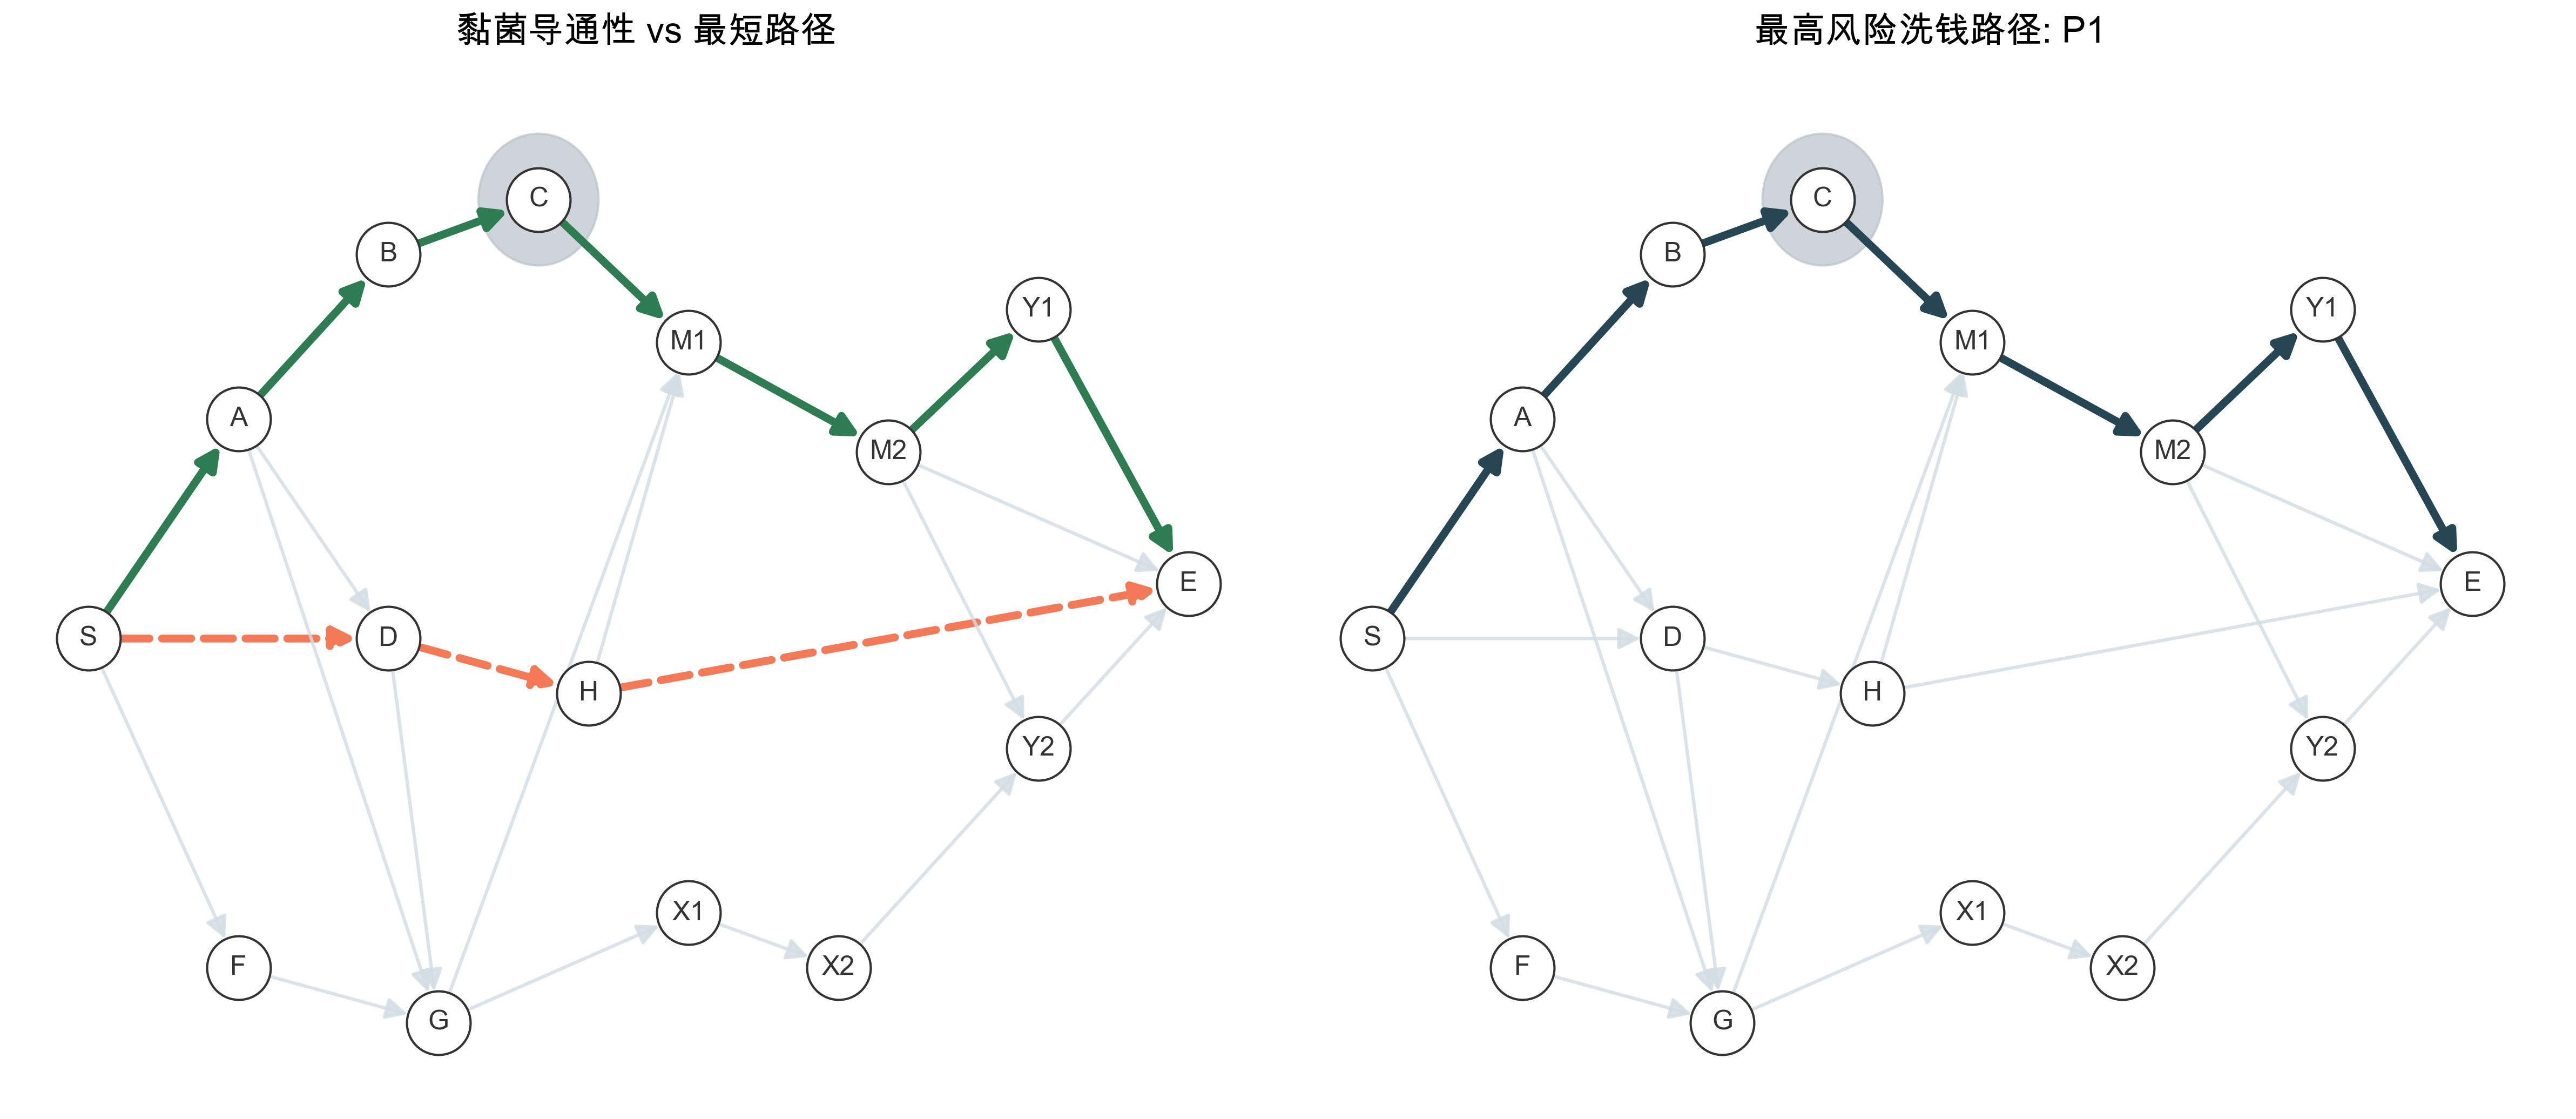
\includegraphics[width=1.0\linewidth]{physarum_network_cn.png}
  \caption{图3：黏菌网络导通性演化与最高风险路径识别}
\end{figure}

\begin{figure}[h]
  \centering
  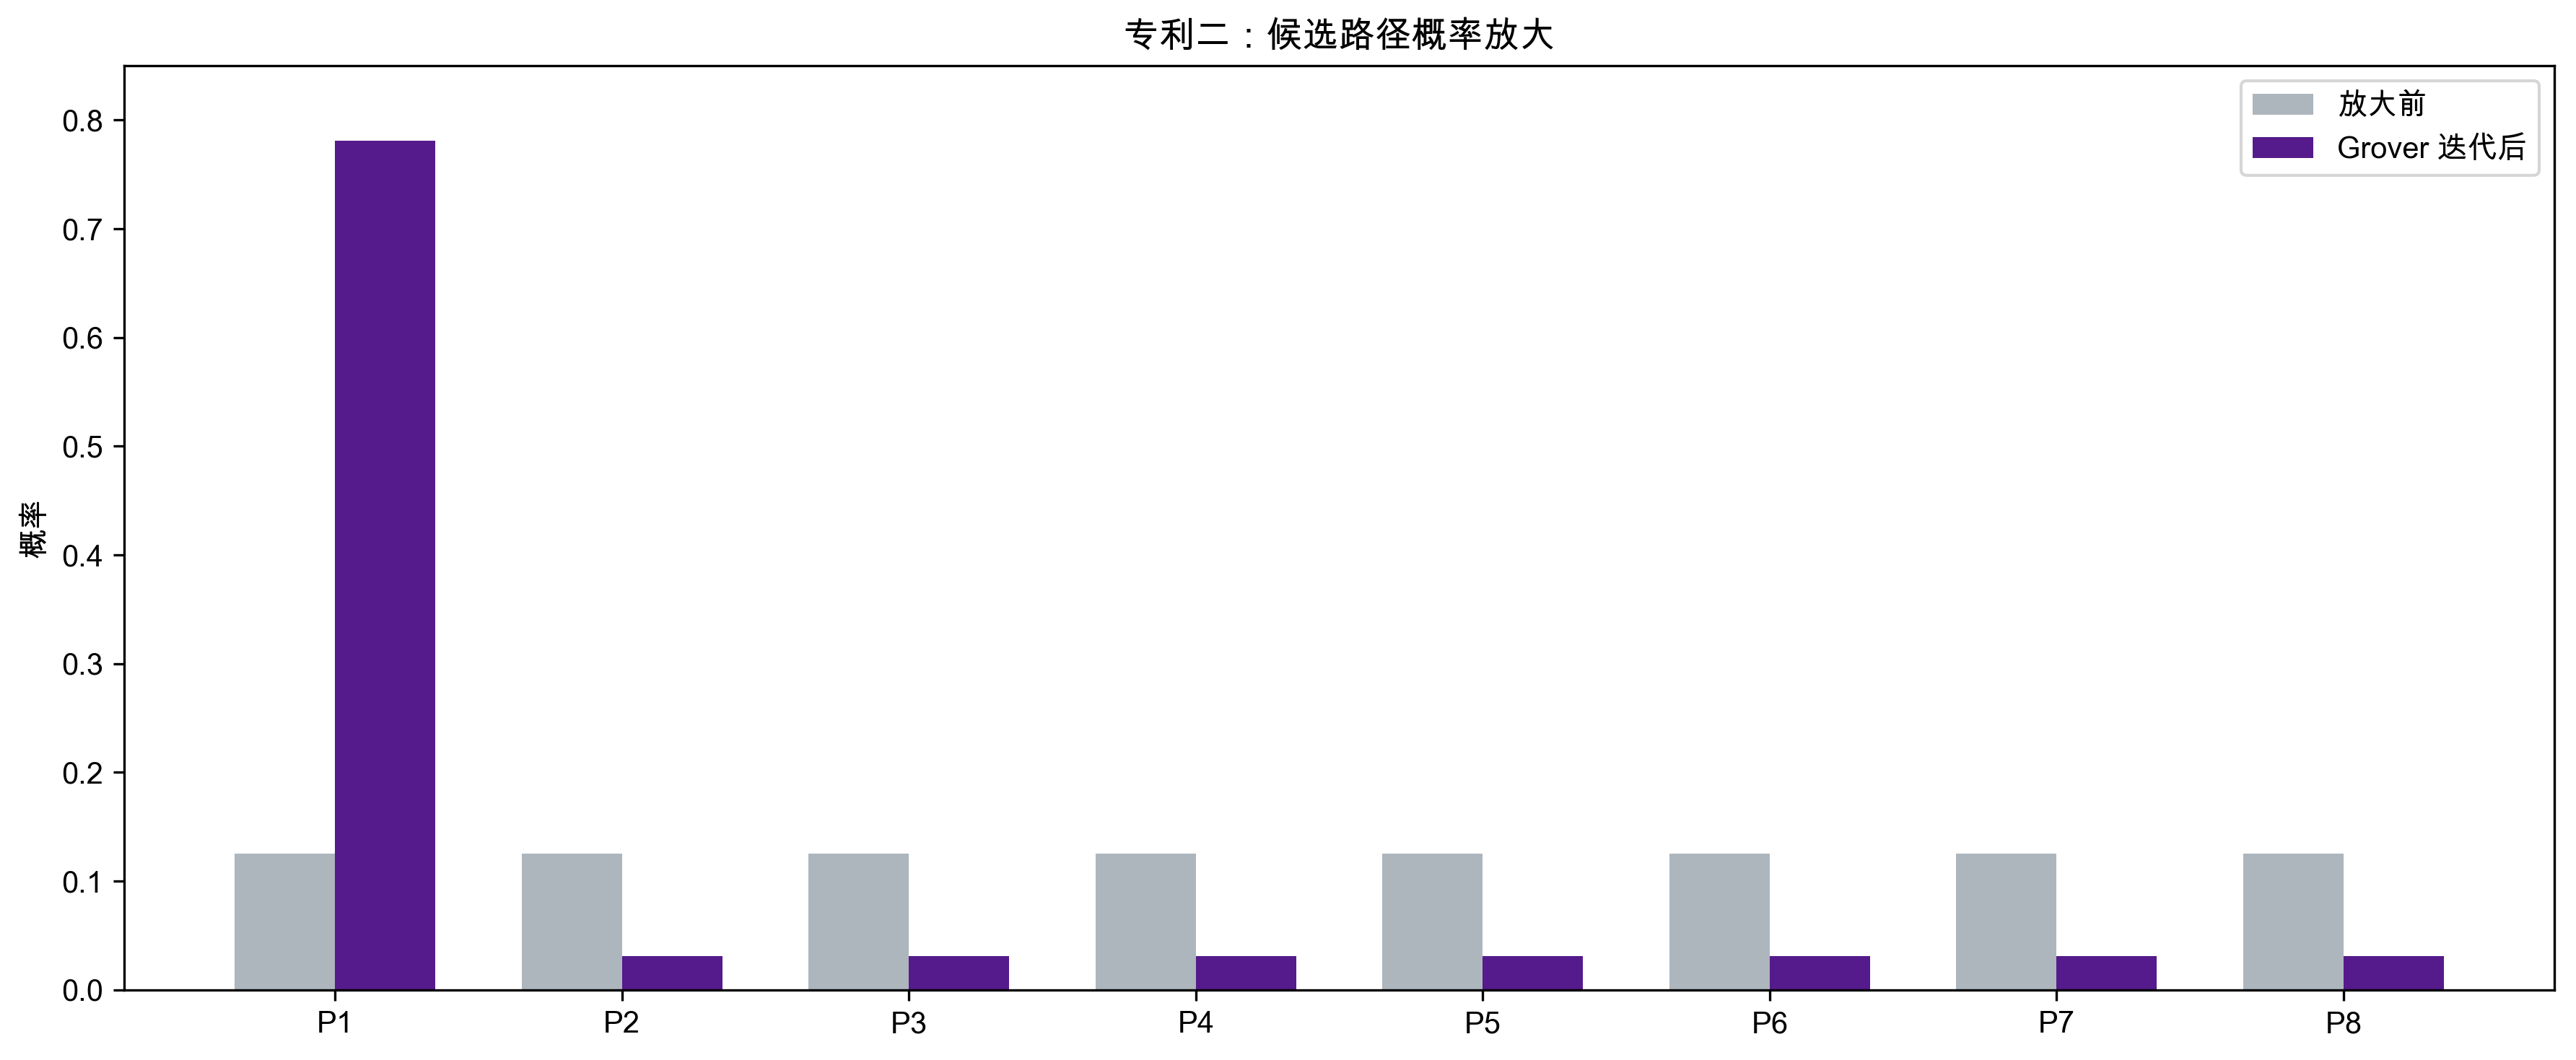
\includegraphics[width=1.0\linewidth]{patent2_grover_circuit_cn.png}
  \caption{图4：Grover 路径放大量子电路图}
\end{figure}

\begin{figure}[h]
  \centering
  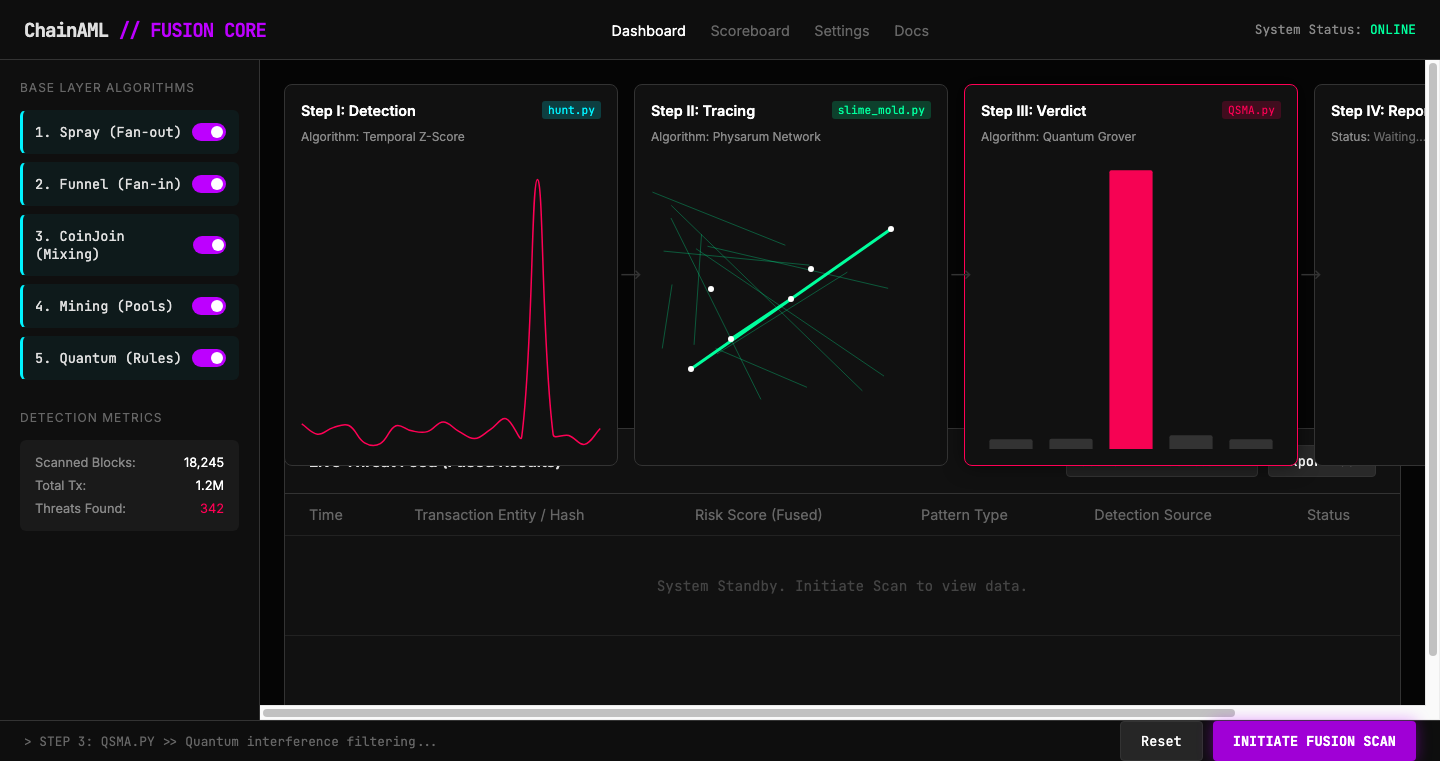
\includegraphics[width=0.9\linewidth]{step2.png}
  \caption{图5：系统 Step II 黏菌路径追踪界面}
\end{figure}

\end{document}

